\documentclass[conference]{IEEEtran}
\input{include/preamble}

\title{
  \fontsize{22}{26}\selectfont
  Fast Synthesis of Power and Temperature Profiles for the
  Development of Data-Driven Resource Managers
}

\author{\input{include/author}}

\begin{document}
  \maketitle

  \begin{abstract}
    We present a methodology and a toolchain for the rapid generation of realistic
power and temperature traces of multiprocessor systems. The target audience of
this work is researchers who develop on-chip solutions that internally rely on
data-driven techniques in order to attain their objectives. Examples of use
cases include proactive power-, energy-, and temperature-aware management
strategies that leverage various machine-learning techniques. In this context,
the availability of a sufficiently large amount of data, which is essential for
learning and prediction and, consequently, for the exploration and exploitation
of research ideas, is rather elusive, to say the least. The presented
methodology and toolchain aim to fulfill this need, that is, to provide profuse
representative data to learn from at the development stage. The overarching goal
is to enable new and facilitate existing studies by making it tractable to
explore novel or revived, highly promising, but potentially data-demanding
techniques for modeling and prediction.

  \end{abstract}

  \begin{IEEEkeywords}
    Computer system,
    machine learning,
    network traffic,
    power,
    simulation,
    temperature,
    workload.
  \end{IEEEkeywords}

  \bstctlcite{IEEEexample:BSTcontrol}

  \section{Introduction and Motivation} \slab{introduction}
  \lettrine[findent=0.4em, nindent=0em]{\textbf{P}}{power} consumption and heat
dissipation are of paramount importance. The two inseparable phenomena dictate
limitations on the usage of electronic devices and severely affect the costs
pertaining to the deployment and maintenance of electronic systems. Power is
essentially energy, and energy translates willingly to service times and
electricity bills. The situation is deteriorated by the fact that a higher level
of power consumption leads to higher temperatures, and higher temperatures
strike back by causing the device to consume even more power. Under these
circumstances, it is no surprise that power and temperature have been in the
limelight for a long time and have no plans on leaving this spot.

\cite{park2015}

Uncertainty.

Machine learning.

Neural networks.

Training data.

Real data.

Synthetic data.

Slow simulators.

Cycle-accurate simulation is an important design tool. It is particularly useful
for the design of individual processing units; however, cycle-accurate
simulation falls short when it comes to large multiprocessor systems. Such
systems are reasonably more complex, which leads to prohibitively large, often
infeasible, simulation times. On the other hand, in order to be properly
addressed, many questions asked in both academia and industry do not need cycle
accuracy. It is important to have an adequate level of abstraction in order to
stay focused on what matters the most to the problem at hand without being
constantly destructed by insignificant or unrelated issues. In such cases, cycle
accuracy can become a serious obstacle.

Sniper raises the level of abstraction \cite{carlson2011}.


  \section{Related Work and Our Contribution}
  The present work is related to simulation techniques. For our purposes, it is
sufficient to distinguish four types of simulation: traffic, performance, power,
and temperature, which are shown in \fref{development}. Here \emph{traffic}
refers to a stream of jobs that lade the system with work, and
\emph{performance} to the system's performance metrics such as the numbers of
executed instructions. We focus on performance, power, and temperature in this
section and on traffic in \sref{traffic}.

A performance simulator that we would like to highlight is Sniper
\cite{carlson2011}. Sniper is aimed at x86-based systems, and it has been
validated against Intel Core 2 and Nehalem architectures. The simulator works at
a higher level of abstraction than the one of cycle-accurate simulators, which
makes its simulation times more affordable. Regarding power simulation, a common
choice is the \sc{McPAT} framework \cite{li2009}. \sc{McPAT} is also capable of
estimating the areas occupied by processing elements, which is useful as this
information is essential for temperature simulation. Architecture-level
temperature simulation is arguably dominated by HotSpot \cite{skadron2004}. A
popular alternative is \sc{3D-ICE} \cite{sridhar2010}, which is more focused on
\sc{3D} structures.

The pipeline assembled from the aforementioned simulators is frequently used in
today's research. However, it is slow and stiff for learning purposes. This is
mainly due to performance simulation and, to a lesser extent, power simulation
as they are considerably time consuming. Temperature simulation has a relatively
small cost compared to the other two.

The need for a systematic assistance in obtaining data for learning-based
undertakings is prominent in the literature. For instance, the study in
\cite{lu2015} proposes a temperature-aware task-allocation strategy based on
reinforcement learning. The authors of that work had to invest time into
developing a custom simulation platform (still based on the above-mentioned
simulators) in order to experiment with their approach. From our perspective,
such auxiliary work should be streamlined.
 \slab{literature}

  \begin{figure*}
  \centering
  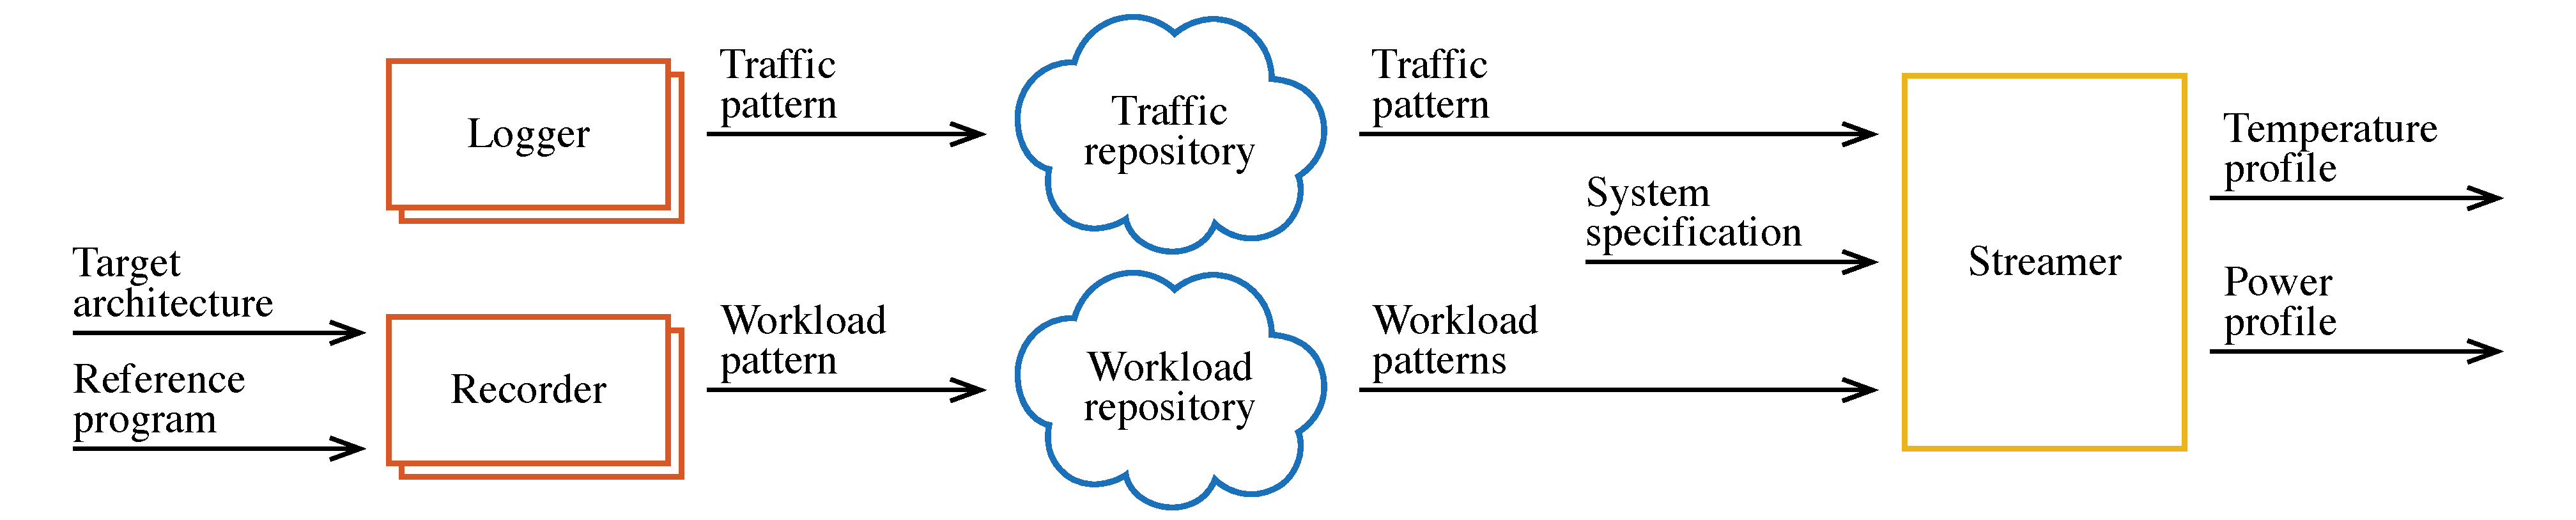
\includegraphics[width=1.0\textwidth]{include/assets/figures/methodology.pdf}
  \caption{The workflow of our methodology.}
  \flab{methodology}
\end{figure*}

  \section{Problem Formulation} \slab{problem}
  Consider an in-design or in-production computer system. The system is composed
of a number of processing elements and is capable of performing a number of
operations. The system receives a stream of user requests or jobs, which it is
supposed to process. Each job implies a certain amount of work to be done and,
thus, a certain amount of power to be consumed and a certain amount of heat to
be dissipated.

Consider now a research project targeted at developing a certain solution for
the system at hand such as a resource manager. Since the importance of power and
temperature is well understood, the solution is required to take them into
account. Suppose further that the solution is to be based on a technique that
learns from the data available at runtime.

Our goal is to develop a toolchain for generating power and temperature profiles
of the system in order to provide the project with plenty of data to experiment
with. The generated profiles should preserve the particularities of job arrivals
and program executions that are present in real life, which is what makes the
subsequent learning meaningful. In addition, the generation process should be
substantially faster than traditional simulations, which is what makes the work
worth doing.


  \section{Methodology} \slab{methodology}
  In this section, we describe the workflow of our methodology and the core models
that the methodology is based on.

\subsection{Traffic}
As described in \sref{problem-formulation}, the system at hand serves a stream
of jobs, which can also be viewed as user requests. The foremost component of
our methodology is then a traffic model, describing how or, rather, when jobs
arrive. This model should satisfy a number of requirements in order to be
practically useful. First of all, the model should be able to capture well the
idiosyncrasies present in real traffic as it establishes a foundation for the
subsequent generation of power and temperature traces. Second, it should be
straightforward to configure the model given a dataset of arrival times serving
as a reference. This last requirement acknowledges the importance of the arrival
data that are at our disposal nowadays due to ubiquitously deployed monitoring
and logging systems.

The seminal work in \cite{leland1994} and subsequent studies have shown that
network traffic exhibits fractal properties such as burstiness, self-similarity,
and long-range dependence, which is very much unlike traditional telephone
traffic. It is well known that traffic models based on the Poisson process
\cite{lifshits2014} are unable to express any of the above properties and,
therefore, drastically departure from reality when it comes to modeling network
traffic. A step in the right direction is to consider the fractional Gaussian
noise \cite{lifshits2014}, which is a self-similar stochastic process. However,
the process is inconvenient to work with from the perspective of a computer
simulator. More concretely, the noise is suited for modeling arrivals per unit
of time but not arrival or inter-arrival times, which are what is typically
needed for simulation. Moreover, even with a proper rescaling and a positive
shift, the process can still take negative values, which is unrealistic.
Finally, the fractional Gaussian noise is a monofractal process; however, real
traffic data often have multifractal structures.

In order to address the aforementioned concerns and enable the generation of
arrival streams exhibiting fractal properties, our methodology employs the
multifractal wavelet model proposed in \cite{riedi1999}, characterizing
positive-valued data with long-range-dependent correlations. To elaborate, we
take a reference time series of arrival times, analyze it by means of the
discrete wavelet transform based on Haar wavelets, and construct a certain
representation of the data, which can then be used for generating random time
series matching the fractal properties of the original one. The model can be
tuned without any reference time series; however, the strength of the technique
is in the rigorous usage of reference data. By doing so, no manual parameter
tuning is needed, and the model gets tailored to the arrival pattern of each
particular problem.

To sum up, we now have a flexible technique for synthesizing arrival times,
which preserves the properties of real arrival data such as burstiness,
self-similarity, and long-range dependence.


\subsection{Workload}
In the previous subsection, we introduced our approach to synthesizing arrival
times, capturing the properties of real arrival data such as burstiness,
self-similarity, and long-range dependence. Now we need to associate a concrete
workload with each arrival time or, equivalently, with each job or user request.
In this regard, there are two main aspects to discuss: the set of workload
candidates and the decision rule used to select a particular candidate for a
particular arrival.

Let us discuss workloads first. Keeping in mind the goal of this work, workloads
should satisfy a number of requirements. First, as emphasized throughout the
paper, we aim to produce realistic power and temperature traces; consequently,
the workloads should represent well the applications/services that the system is
supposed to provide to the end user. Second, a workload should be fast to
evaluate, which, in our context, refers to computing the power consumption of
that workload.

The particularities of the power consumption of a computer program are hard to
fabricate. A sequence of random numbers taken out of thin air will not do the
trick as programs have certain algorithmic structures. For instance, a program
might traverse a number of phases, and each phase might involve a number of
distinctive computations, shaping the corresponding power and temperature
profiles. Such features are important to preserve in order to make the
subsequent experimentation with machine-learning techniques and alike
meaningful.

With the above concern in mind, the workload-modeling part of our methodology is
founded on full-system simulations of representative programs. However, if we
had incorporated such simulations directly into our workflow, it would have
defeated the purpose of our work since, as motivated in \sref{introduction},
detailed simulations are too time consuming. Instead, we propose the use of
high-level recordings. To elaborate, we run each reference program under an
adequate simulator, capable of modeling the target platform, and record the
information that is needed for our data generation.\footnote{Such a technique is
similar in spirit to PinPlay \cite{patil2010}, which is a tool for recording and
replaying an execution of a program on the instruction level.} From our
experience, performance and power simulation is by far the largest expense on
the way to temperature, and, therefore, we propose to record is power directly,
eliminating this expense all together. The result of the above procedure is a
catalog of power traces corresponding to real programs, which we shall refer to
as power patterns.

Simulations obviously take time; however, they should be done only once.
Moreover, such a catalog of real power patterns can be populated and maintained
online by the research community so that the patterns are at a one-click
distance from any single researcher, and no expensive simulation is needed. The
role of the catalog could be similar to the one played by the benchmark suites
commonly used in research now-a-days, such as \sc{PARSEC} \cite{bienia2011} and
\sc{SPEC CPU2006} \cite{cpu2006}.

Now, it should be clear that, by recording power directly, we make a significant
trade-off: many details related to programs' executions have been discarded in
order to gain speed. What has been baked in into recordings cannot be to altered
at the usage/replay stage in general.

In our experiments, we use the applications from two benchmark suites, namely,
from \sc{PARSEC} and \sc{SPEC CPU2006}, which were mentioned earlier.


\subsection{Performance}
Sniper \cite{carlson2011}.
\begin{table}
  \caption{Target architecture}
  \begin{tabular*}{\linewidth}{=L{70pt}l}
    \toprule
    Component    & Description \\
    \midrule
    Core         & 2660 MHz, 1.2 V \\
    L1-I/D cache & 32 KB, 4-way, LRU, private \\
    L2 cache     & 256 KB, 4-way, LRU, private \\
    L3 cache     & 8192 KB, 16-way, LRU, one per four cores \\
    \bottomrule
  \end{tabular*}
  \tlab{target}
\end{table}
% vim: nowrap tw=0


\subsection{Power}
\sc{McPAT} \cite{li2009}.

\subsection{Temperature}
HotSpot \cite{skadron2004}.
\sc{3D-ICE} \cite{sridhar2010}.
The solver is based on exponential integrators \cite{hochbruck2010},
\cite{ukhov2012}.


  \section{Toolchain} \slab{toolchain}
  An important part of this work is a toolchain embodying the methodology. The
toolchain has been implemented in the Rust programming language
\cite{rust}.\footnote{Rust is a systems programming language developed by
Mozilla Research and thousands of independent contributors from all around the
world. Rust provides memory safety without garbage collection, concurrency
without data races, abstractions without overhead, and stability without
stagnation.} It consists of a number of command-line tools, and the tools are
composed of a number of stand-alone packages. The toolchain also makes use of
third-party software, including the state-of-the-art simulators introduced in
\sref{prior-work}. Regardless of the origin, each component toolchain is open
source. The code written by us is distributed under the \sc{MIT} license
\cite{mit} and is available at \cite{sources}.

The main programs of our toolchain are called Recorder and Streamer, and we
shall describe their architectures in the following subsections. Before we
proceed, let us remind that collecting reference arrival data (series of arrival
times) is outside of the scope of this work (see \sref{traffic}).

\subsection{Recorder} \slab{recorder}
\begin{figure}
  \centering
  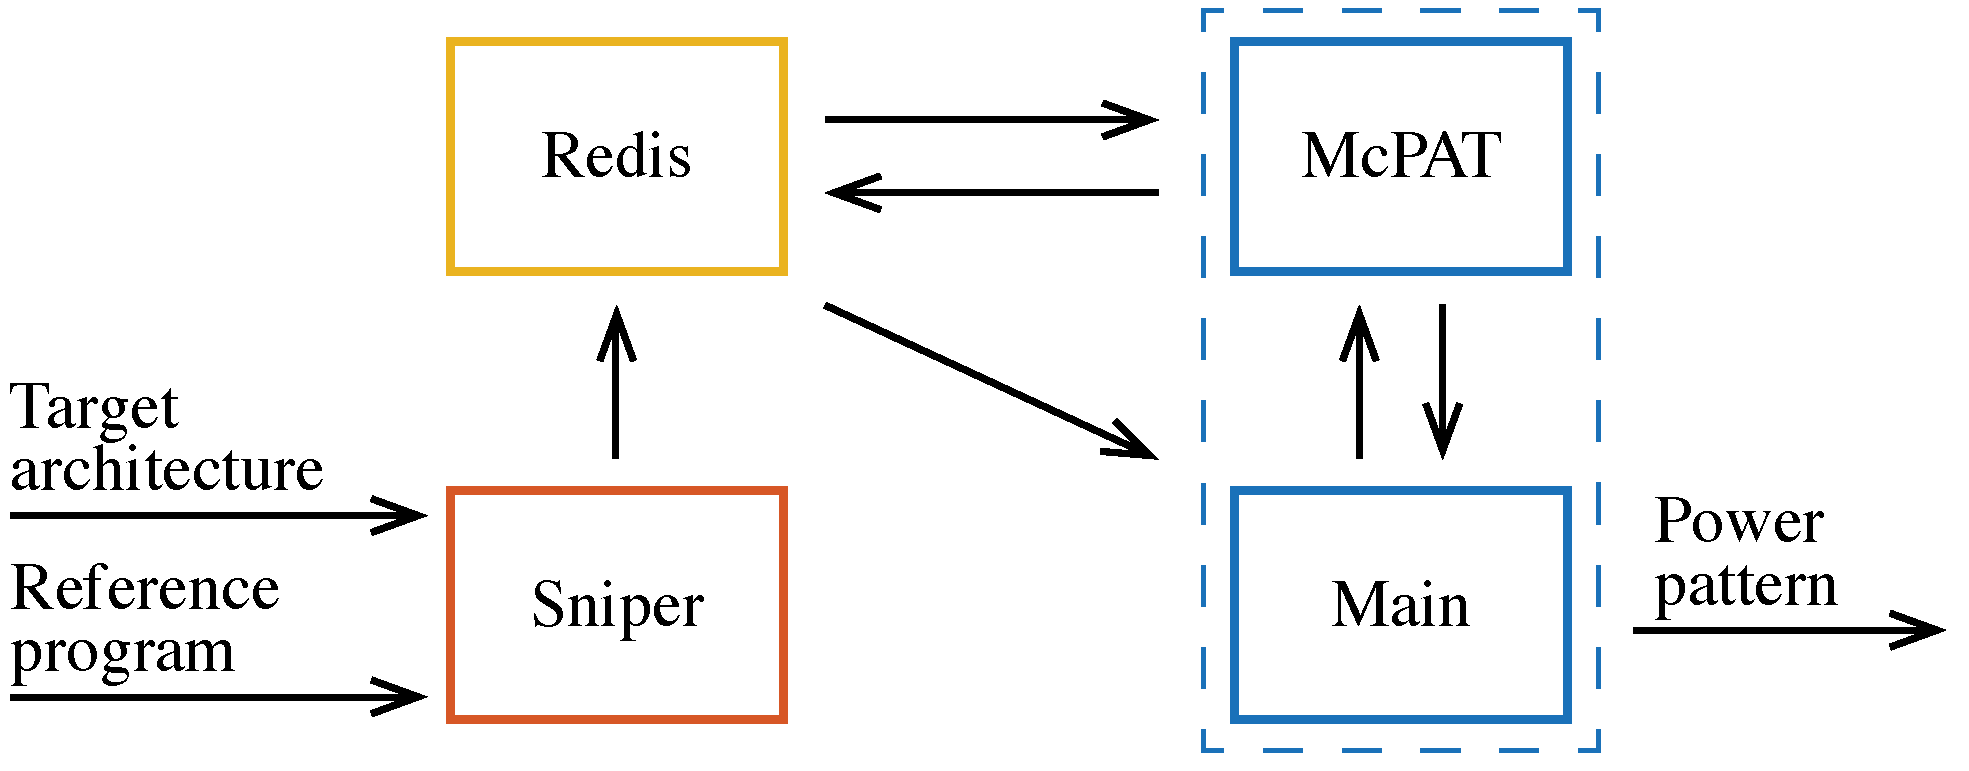
\includegraphics[width=1.0\columnwidth]{include/assets/figures/recorder.pdf}
  \caption{The recording infrastructure.}
  \flab{recorder}
\end{figure}

As the name suggests, the purpose of \recorder\ is recording. More specifically,
the tool records power traces, which are needed as an input to \streamer. The
recording infrastructure is depicted in \fref{recorder}.

Sniper \cite{carlson2011}.
\begin{table}
  \caption{Target architecture}
  \begin{tabular*}{\linewidth}{=L{70pt}l}
    \toprule
    Component    & Description \\
    \midrule
    Core         & 2660 MHz, 1.2 V \\
    L1-I/D cache & 32 KB, 4-way, LRU, private \\
    L2 cache     & 256 KB, 4-way, LRU, private \\
    L3 cache     & 8192 KB, 16-way, LRU, one per four cores \\
    \bottomrule
  \end{tabular*}
  \tlab{target}
\end{table}
% vim: nowrap tw=0


The key-value storage is Redis \cite{redis}. The database is SQLite
\cite{sqlite}.

\sc{McPAT} \cite{li2009}.


\subsection{Streamer} \slab{streamer}
\begin{figure}
  \centering
  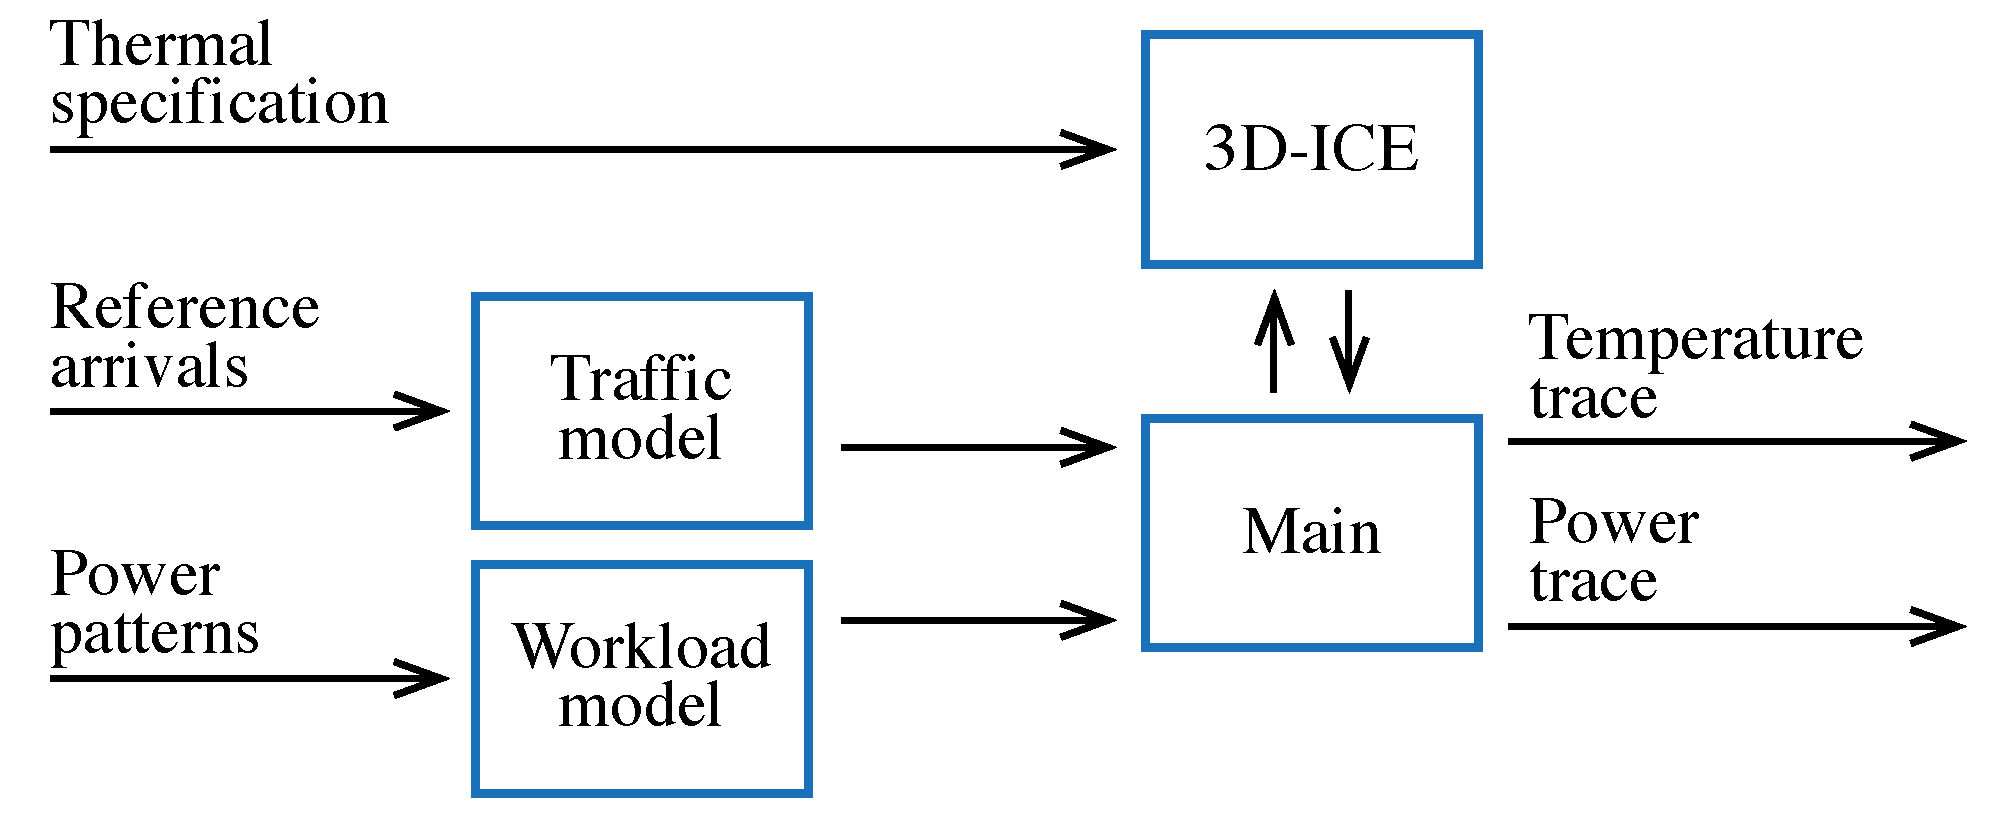
\includegraphics[width=1.0\columnwidth]{include/assets/figures/streamer.pdf}
  \caption{The streaming infrastructure.}
  \flab{streamer}
\end{figure}

The streaming infrastructure is depicted in \fref{streamer}.

HotSpot \cite{skadron2004}.
\sc{3D-ICE} \cite{sridhar2010}.
The solver is based on exponential integrators \cite{hochbruck2010},
\cite{ukhov2012}.



  \balance

  \section{Experimental Results} \slab{result}
  This section illustrates the performance of the toolchain presented in
\sref{toolchain}. The experiments that are reported below were conducted on a
\sc{GNU}/Linux machine equipped with 16 \sc{CPU}s Intel Xeon E5520 2.27~\sc{GH}z
and 24~\sc{GB} of \sc{RAM}.

In order to obtain real-life traffic patterns for our experiments, we used a
data set published by Google in 2011 \cite{reiss2011}. The data set contains the
usage data of a large computer cluster over a month period. We downloaded the
table tracking the life cycle of the jobs submitted to the cluster and extracted
the time stamp of the first event related to each job. As a result, there were
around 670\,000 arrival times available, which we used for fitting the traffic
model as it is described in \sref{traffic}.

A set of workload patters was obtained by simulating and recording (via our
infrastructure shown in \fref{recorder}) the programs from the popular
\sc{PARSEC} \cite{bienia2011} and \sc{SPEC CPU2006} \cite{cpu2006} benchmark
suites; the former contains 13 programs, and the latter 29 programs. The
architecture used in these simulations is Intel's Nehalem-based Gainestown
series; Sniper is shipped with a configuration for this architecture
(\tt{nehalem.cfg} and \tt{gainestown.cfg}), and we used it without any changes.

All the reference data that we collected and processed to make them suitable for
our toolchain are available at \cite{sources}.

\subsection{Recording}
\begin{table}
  \begin{threeparttable}
    \caption{Recording of the \sc{PARSEC} benchmark suite}
    \begin{tabular*}{\linewidth}{=L{43pt}-R{24pt}-R{24pt}-R{24pt}-R{17pt}-R{17pt}-R{17pt}}
      \toprule
      & \multicolumn{3}{c}{Recording time, m} & \multicolumn{3}{c}{Simulated time, s} \\
      Program       & S & M & L & S & M & L \\
      \cmidrule( r){1-1}
      \cmidrule(l ){2-4}
      \cmidrule(l ){5-7}
      blackscholes  &  10.77 &  44.21 & 0 & 0.08 & 0.31 & 0 \\
      bodytrack     &  30.58 & 120.04 & 0 & 0.19 & 0.80 & 0 \\
      canneal       &  36.90 & 104.52 & 0 & 0.17 & 0.63 & 0 \\
      dedup         &  81.26 & 208.80 & 0 & 1.66 & 2.86 & 0 \\
      facesim       & 760.59 & 790.80 & 0 & 8.54 & 8.47 & 0 \\
      ferret        &  49.67 & 159.19 & 0 & 0.49 & 1.32 & 0 \\
      fluidanimate  &  46.55 & 131.00 & 0 & 0.59 & 1.43 & 0 \\
      freqmine      &  74.45 & 292.28 & 0 & 0.72 & 2.75 & 0 \\
      raytrace      & 253.23 & 341.32 & 0 & 0.28 & 0.75 & 0 \\
      streamcluster &  44.57 & 172.50 & 0 & 0.36 & 1.45 & 0 \\
      swaptions     &  35.20 & 140.02 & 0 & 0.24 & 0.97 & 0 \\
      vips          &  94.00 & 293.51 & 0 & 0.57 & 1.71 & 0 \\
      x264          &  29.36 & 155.16 & 0 & 0.19 & 1.05 & 0 \\
      \bottomrule
    \end{tabular*}
    \tlab{recording}
    \begin{tablenotes}
      \item Note the difference in the units of measurement: the recording time
      is in minutes, and the simulated time is in seconds. S, M, and L stand
      for ``small,'' ``medium,'' and ``large,'' respectively, and signify input
      size.
    \end{tablenotes}
  \end{threeparttable}
\end{table}
% vim: nowrap tw=0

In the above, we outlined how the reference workload data were harvested using
Recorder and the infrastructure around it (recall \sref{recorder} and
\fref{recorder}). Let us now elaborate on the performance characteristics of
that recording process.

The benchmark suite that we shall look at is \sc{PARSEC}. Our findings are
summarized in \tref{recording}. \sc{PARSEC} provides several choices of inputs
to the programs, and each program was recorded with three different inputs,
namely, with the ones classified as small, medium, and large. There are two
types of information shown in \tref{recording}: recording time (in hours), which
is the time that was taken to simulate and record the programs, and simulated
time (in seconds), which is the time that the programs would have taken in real
life. The sampling interval used in all the experiments was one millisecond.

Each input class was recorded in a single batch: all 13 programs were simulated
at the same time using 13 Sniper processes, which is explained and motivated in
\sref{streamer}. Consequently, the total recording time with respect to each
batch is dictated by the program that took the most time to finish. For small
and medium inputs, this program was \texttt{facesim}, which took approximately
13 hours in both cases. The simulated times of \texttt{facesim} indicate that
\sc{PARSEC} actually has only one input size for this particular program.
Regarding large inputs, \texttt{freqmine} finished last; more concretely, the
program took 18 hours. As an aside for the interested reader, the simulated and
recording times of \sc{SPEC CPU2006} (not shown) were an order of magnitude
larger than the ones of \sc{PARSEC}.

It can be seen in \tref{recording} that the throughput in terms of simulated
time is (expectedly) low: roughly speaking, two--three hours of recording time
amounts to one second of simulated time. However, it is important to realize
that these are one-time expenses in our methodology; the situation would be much
worse if one had to perform such simulations all the time (see \sref{workload}).
Another important aspect to note is that the observed recording times have been
substantially reduced by the choice of performance simulator---Sniper is based
on novel simulation ideas \cite{carlson2011}---and the parallelization strategy
and caching mechanism described in \sref{streamer}.


\subsection{Streaming}
\setlength{\tabcolsep}{4pt}
\begin{table}
  \begin{threeparttable}
    \caption{Streaming (synthesis of power and temperature profiles)}
    \begin{tabular*}{\linewidth}{=L{50pt}-R{40pt}-R{40pt}-R{40pt}-R{40pt}}
      \toprule
      \multirow{2}{*}{\parbox{50pt}{Synthesized time (seconds)}} & \multicolumn{4}{c}{Synthesis time (seconds)} \\
      & $4 + 1$ & $8 + 2$ & $16 + 4$ & $32 + 8$ \\
      \cmidrule( r){1-1}
      \cmidrule(l ){2-5}
         10 &   0.24 &   0.40 &   0.67 &   1.13 \\
        100 &   2.11 &   3.66 &   6.18 &  10.19 \\
       1000 &  20.59 &  37.47 &  64.58 & 104.00 \\
      10000 & 214.98 & 394.84 & 598.89 & 984.59 \\
      \bottomrule
    \end{tabular*}
    \tlab{streaming}
    \begin{tablenotes}
      \item \hspace{-0.70em}``$M + N$'' stands for $M$ cores and $N$ L3 caches.
      Every four cores have a shared L3 cache; therefore, it holds that
      $N = M / 4$.
    \end{tablenotes}
  \end{threeparttable}
\end{table}
% vim: nowrap tw=0

Let us turn to Streamer, which corresponds to the data-synthesis stage (recall
\sref{streamer} and \fref{streamer}). Our objective in this subsection is to
study the scalability of the tool as measured by synthesis time, which is the
time that is needed for the tool to synthesize power and temperature profiles
under certain conditions or requirements. In these experiments, workload
patterns are assigned to job arrivals randomly, and a simple
first-in-first-served scheduling policy is assumed; both are the default but
easily replaceable options used by the toolchain.

The preformed experiments are consolidated in \tref{streaming}. We report our
synthesis time along two axes: synthesized time (rows) and platform size
(columns). The former is analogous to simulated time, and the latter represents
different platforms as follows. Each considered platform is composed of a number
of cores, and there is a single L3 cache for every four cores; both cores and
caches are referred to as processing elements. Platform size is defined as the
number of processing elements, and it is denoted by ``$M + N$'' in
\tref{streaming} where $M$ and $N$ are the numbers of cores and L3 caches,
respectively.

Unlike the throughput of simulation (discussed in the previous subsection), the
throughput of synthesis in terms of synthesized time is very high, which is well
supported by \tref{streaming}. To give an example, it takes Streamer around a
minute to produce power and temperature data that are worth around 17 minutes of
runtime of a computer system with 16 cores, which would be practically
infeasible to achieve with full-fledged simulations (refer to the results given
in \tref{recording}).

Another observation made from \tref{streaming} is that synthesis time scales
linearly with respect to the length of the time span being synthesized
(synthesized time), and the same can be concluded regarding the other dimension,
platform size. The growth with respect to platform size is due to the increasing
complexity of the underlying thermal \sc{RC} circuit used for temperature
simulation; thermal circuits are elaborated on in \sref{streamer}.


To summarize, the results reported in \tref{recording} motivate our work and
communicate well the message of this paper: the speed of the state-of-the-art
simulators is severely onerous for the purpose of experimenting with
machine-learning techniques. The core problem is that such techniques typically
require lots of data (long execution traces); moreover, these data might need to
be recalculated each time a parameter changes such as the parameterization of
the scheduling policy used. The results in \tref{streaming} show that the
proposed approach can efficiently tackle this problem by taking the data burden
away and, hence, making it easier to experiment with data-driven techniques.


  \section{Conclusion} \slab{conclusion}
  In this paper, we have emphasized the need for developing tools for the design
of computer systems with data-driven applications in mind. We have argued that
the techniques which capitalize on learning from runtime data have special
requirements, and that the state-of-the-art simulators are unable to fulfill
them due to their prohibitively large simulation times.

Acknowledging the importance of power and temperature for the design of computer
systems, we have developed a methodology for fast generation of power and
temperature profiles of such systems, which preserve the idiosyncrasies of their
real-life counterparts. Following the methodology, we have implemented and
open sourced a toolchain, which has been assessed and shown to have a high
computational throughput.


  \bibliographystyle{IEEEtran}
  \bibliography{IEEEabrv,include/bibliography}
\end{document}
